%!TEX root = main.tex
\section{Protocol Overview}

\paragraph{Notation.} We use $\signed{m}{\pk}$ to denote a message signed by the secret key of $\pk$.

\paragraph{Overview.}

There are three types of players:

\begin{itemize}
    \item Any trust servers $(S_1, \dots, S_\ell)$ running~\cref{proto:server}.
    \item Aggregators (each with an SGX enclave) $(A_1, \dots, A_m)$ running~\cref{proto:agg}.
    \item Users (each with an SGX enclave) $(U_1, \dots, U_n)$ running~\cref{proto:user}.
\end{itemize}

\newcommand{\schedstate}{\mathsf{State}_\text{sched}}
\newcommand{\schedmsgin}{m_\text{in}}
\newcommand{\schedmsgout}{m_\text{out}}
\newcommand{\schedround}{r_\text{sched}}

\begin{figure}
\protocol{Protocol of a user $U_i$}{
\textbf{State:} \\
\begin{itemize}[leftmargin=*]
    \item $(\sk, \pk)$ a pair of keys generated in an enclave. $\pk$ is published in an attestation. $\sk$ is sealed to persistent storage for backup.
    \item Pair-wise keys with all servers: $K_{i,j} \in \bin^\secpar$ for $j\in [\ell]$.
\item Round counters $\schedround$ for the scheduling protocol and $r$ for the normal communcation rounds. Counters start with $0$ and get incremented as specified below.
\item Scheduling state $\schedstate:=\bot$
\end{itemize}
\textbf{Registration:} \\
\t $U_i$ talks to all servers to generate keys and store them. $U_i$ also registers the public key of her local enclave $\enclavekey$. \\[2mm]
\textbf{Scheduling and submission:} \\
$U_i$ runs scheduling along with normal message submission. Let $M$ be the message $U_i$ wants to send in the current round (and $M$ is all zeroes if $U_i$ is not scheduled to send).
\begin{itemize}
    \item Schedule: Calls $(\schedmsgout, \schedstate') = schedule(\schedmsgin, \schedstate)$. Increment $\schedround$ by $1$. If $\schedround=R$, set $\ticket=\schedstate'$, $\schedstate=\bot$, and $\schedround=0$. Otherwise set $\schedstate=\schedstate'$.
    \item Encrypt: $U_i$ calls $M=prepare(\ticket, r, m)$. See text for a description of $prepare$.
    \item Submit: $U_i$ submits $\schedmsgout \| M$ to one or more of the aggregators. Increment $r$ by $1$.
\end{itemize}
\textbf{Output:} \\
Wait to receive the final outcome from aggregators $(r, \vec{m}, \vec{\sigma})$.
}
\caption{User protocol}
\label{proto:user}
\end{figure}


\subsection{User protocol}

To register, each user generates a key pair $(\sk, \pk)$ using an enclave where $\pk$ is published in an attestation and $\sk$ is sealed (encrypted by a key known only to the enclave) to persistent storage for backup.

\subsubsection{Registration}
To join the DC net for communication, a user first registers with the server committee. To do so, the user sends the public key of her local enclave $\enclavekey$ and negotiates pair-wise keys with all servers: $K_{i,j} \in \bin^\secpar$ for $j\in [\ell]$.


\subsubsection{Scheduling}

If two participants in a DC net send in the same round---either accidentally or maliciously---their messages collide and the broadcast is disrupted. Therefore, it is essential to coordinate among senders so that ideally only one participant sends in a given round. We refer to this process as {\em scheduling}.

There are generally three approaches to solve this problem. The first is to have participants send {\em reservation messages} to reserve future rounds and resolve collisions. The second approach is to defer the problem of collision to the communication phase, i.e., to {\em resolve} collisions when they happen instead of to prevent them. The third approach is to use secure MPC to compute a random slot assignment. We adopt the first approach and use the footprint scheduling protocol~\cite{}. \fanz{what are the rational: simple, efficient (no MPC or ZKP), can be done on top of DC net. What else?} Compared to the original reservation protocol in~\cite{chaum}, footprint scheduling significnatly reduces the length of reservation vectors. Because the scheduling messages are so short, they can be piggybacked on normal messasges, like in~\cref{fig:message}.

% The ideal functionality of scheduling takes as input a list $\mathcal{U}$ of users who wish to speak in the next $S$ rounds, outputs a list of $S$ identities $(U_1, U_2, \dots, U_S)$ such that $U_i \in \mathcal{U}$, which schedules $U_i$ to speak at the $i$th round. Note that if $|\mathcal{U}|<S$, the output may contain duplicated identities.

% We use footprint scheduling~\cite{} to assign participants to rounds, so that ideally only one participant sends messages in a given round. Footprint scheduling is done $R=\log(N)$ rounds~\cite{}. We set parameters to ensure $R \le S$ so that scheduling rounds can be piggyback on normal message, like in~\cref{fig:message}.

\paragraph{Scheduling in an enclave.} However, footprint scheduling does not prevent active malicious participants from disruppting the communication by just not observing the protocol. Therefore we run the footprint scheduling in an enclave.

User's enclave has a single API for scheduling: $schedule(\schedmsgin, \schedstate) \to (\schedmsgout, \schedstate')$, which takes as input the previous broadcast messages and state, and outputs a new scheduling messages to be sent through the DC net and an updated state. $\schedstate=(i, slots, footprints)$ where $i$ is the scheduling round number, $slots$ the slots being reserved, $footprints$ the current footprints used to detect collision. Since the scheduling termintes in exactly $R$ rounds (a parameter). The $\schedstate$ of the final round becomes the ticket for the user to send in rounds in $\schedstate.slots$.

\begin{figure}[H]
    % \includegraphics[page=6,width=\columnwidth]{all-images.pdf}
    \centering
    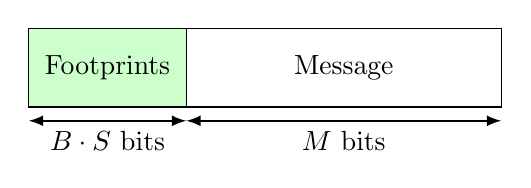
\begin{tikzpicture}[
            scheduling/.style={draw=black, fill=green!20},
            bigbrace/.style={decorate,decoration={brace,amplitude=5pt,raise=4pt}},
            bigbracemirror/.style={decorate,decoration={brace,mirror,amplitude=5pt,raise=4pt}},
        ]
        \draw[scheduling] (0, 0) rectangle (2, 1);
        \draw (2, 0) rectangle (6,1);
        \draw (1, .5) node[align=center] {Footprints} +(3, 0) node {Message};
        \draw[<->, thick, >=latex, yshift=-5pt] (0.0, 0) -- (2, 0) node [black,midway,below] {$B\cdot S$ bits};
        \draw[<->, thick, >=latex, yshift=-5pt] (2, 0) -- (6, 0) node [black,midway,below] {$M$ bits};
    \end{tikzpicture}
    \caption{A DC net message consisting of a footprints for scheduling  (green part; up to $B\cdot S$ bits) and regular message}
    \label{fig:message}
\end{figure}

\paragraph{Submitting.} User's enclave has a single API for constructing messages to be broadcast: $prepare(\ticket, r, m, \schedmsgout)\to \signed{M}{\pk}$. The enclave verifies the ticket $\ticket$ and checks $m$ is zeroes unless $U_i$ is authorized to submit in round $r$. The enclave computes keys $K_{i}=\oplus_{j=1}^{\ell} \prg(K_{i,j}\|r)$ and outputs $M=(U_i, r, c_i=m \xor K_i,\schedmsgout)$.

\subsection{Server protocol}


\begin{figure}
    \protocol{Protocol of a server $S_i$\fanz{no need for SGX unless for defense-in-depth?}}{
        \textbf{Finalize:} \\
        \begin{itemize}[leftmargin=*]
            \item Upon receiving from all aggregators or the round closure deadline has passed, the server $S_j$ forms a list $L_j$ of all client identifiers included in aggregator messages. Broadcast $L_j$ to other servers.
            \item Given all servers' lists, the servers determines a list $L_r$ of clients who submitted in round $r$. Talking to the aggregator if needed (e.g., to retrieve messages not aggregated), all servers reach agreement on the final aggregated message $c_r = \bigoplus_{i \in L_r} c_i$.\fanz{alternatively, we could have aggregators to reach consensus first, and servers just take the largest aggregation set as $L_r$.}
            \item Each server $S_j$ computes her pad $K_{S_j}=\bigoplus_{i\in L_r}{K_{i,j}}$ and broadcast $\signed{r, K_{S_j}, L_r}{\pk_{S_j}}$ to connected aggregators.\fanz{in Dissent this is sent to the clients directly but in our setting the server doesn't interact with clients directly.}
        \end{itemize}
    }
    \caption{server protocol}
    \label{proto:server}
\end{figure}

\subsection{Aggregator}


\begin{figure}
    \protocol{Protocol of an aggregator $A$ (and her enclave)}{
        \textbf{State:} \\
        \begin{itemize}[leftmargin=*]
            \item $(\sk_A, \pk_A)$: key pair. Ditto.
            \item A mapping $(r, \mathcal{U}, c)$ storing the aggregated messages so far (for round $r$).
        \end{itemize}
        \textbf{Aggregate}($U_i, c_i$): \\
        \t Retrieve $(r, \mathcal{U}, c)$ from local storage. If $U_i\in\mathcal{U}$, ignore and return. If not, store $(r, U_i, c_i)$ for reasons that will become clear shortly, set $\mathcal{U}:=\set{U_i} \cup \mathcal{U}$ and $c:=c_i \xor c$. Broadcast $(r,\mathcal{U}, c)$ to other aggregators. When $|\cal U|$ is big enough or a timeout has passed, $A$ sends $(r,\mathcal{U}, c)$ to all servers. \\
        \textbf{Catchup}: \\
        \t When receiving $(r,\mathcal{U}', c')$ from a peer aggregator $A'$, catch up if needed. \fanz{$A$ can't simply xor with $c'$ if $U$ overlaps with $U'$. But it's not hard either given both are honest.} \\
        \textbf{Finalize:} \\
        \t After receiving signed pads $(r, K_{S_j}, L_r)$ from all servers, $A$ computes $m=c_r \xor K_{S_1} \xor K_{S_2} \dots \xor K_{S_\ell}$, signs it, and sends to all connected clients. Proceed to round $r+1$.
    }
    \caption{aggregator protocol\fanz{enclave is stateless. state is stored out of aggregator.}}
    \label{proto:agg}
\end{figure}